\subsection{Многолучевая интерференция}


\textbf{Прошедшая волна}.
Обозначим через $R$ коэффицент отражение света от границы раздела пластинки с воздухом. При отсутсвии поглощения $(1-R)$ проходит через границу, если среды по обе стороны одинаковы, то и $R$ будут одинаковы. Пусть свет монохроматичен
Пусть интенсивность света $I_0$, тогда интенсивности прошедших пучков будут
\begin{equation*}
    I_{1'} = (1-R)^2, \hspace{5 mm} 
    I_{2'} = R^2(1-R)^2 I_0, \hspace{5 mm} 
    I_{3'} = R^4 (1-R)^2 I_0, \hspace{5 mm}  \ldots
\end{equation*}
а соответсвеющие вещественные амплитуды
\begin{equation*}
    a_{1'} = (1-R) a_0, \hspace{5 mm} 
    a_{2'} = R(1-R) a_0, \hspace{5 mm} 
    a_{3'} = R^2(1-R) a_0, \ldots .
\end{equation*}
Амплитула прошедшей волны представится убывающей геометрической прогрессией
\begin{equation*}
    \sub{a}{d} = a_0 (1-R)\left[1 + R e^{-i \Phi} + R^2 e^{-2i \Phi} + \ldots\right],
    \hspace{5 mm} 
    \Phi = k \Delta = \frac{4 \pi}{\lambda} n d \cos \psi,
    \hspace{0.5cm} \Rightarrow \hspace{0.5cm}
    \sub{a}{d} = \frac{1-R}{1-R e^{-i\Phi}} a_0.
\end{equation*}
где $\Phi$ -- разность фаз между соседними пучками.  Интенсивность прошедшей волны
\begin{equation*}
    \sub{I}{d} = \frac{(1-R)^2}{|1-R e^{-i \Phi}|^2} a_0^2 = \frac{(1-R)^2}{(1-R)^2 + 4 R \sin^2 (\Phi/2)} I_0,
\end{equation*}
что позволяет сделать некоторые выводы. 



\textbf{Отраженная волна}. Аналогичный расчёт приведет к
\begin{align*}
    &I_1 = R I_0, 
    &I_2 = R(1-R)^2 I_0, 
    &&I_3 = R^3 (1-R)^2 I_0, 
    &&\ldots, \\ 
    &a_1 = \sqrt{R} a_0, 
    &a_2 = - \sqrt{R} (1-R) a_0, 
    &&a_3 = - \sqrt{R} R (1-R) a_0, 
    &&\ldots,
\end{align*}
где знак в $a$ -- следставие появления $\lambda/2$. Резуьтирующая амплитуда будет иметь вид
\begin{equation*}
    a_r = \sqrt{R} a_0 - \sqrt{R} (1-R) a_0 e^{-i \Phi} \left[
        1 + R e^{- i \Phi} + R^2 e^{-2i \Phi} + \ldots
    \right],
    \hspace{0.5cm} \Rightarrow \hspace{0.5cm}
    I_r = \frac{4 R \sin^2 (\Phi/2)}{(1-R)^2 + 4 R \sin^2(\Phi/2)} I_0, 
\end{equation*}
где всё также $\Phi = k \Delta = \frac{4 \pi}{\lambda} n d \cos \psi$.


При $R \ll 1$ увидим случай двулучевой интерференции, при $R \approx 1$ уже интереснее (рис. \ref{fig:piks}). 
\begin{figure}[ht]
    \centering
    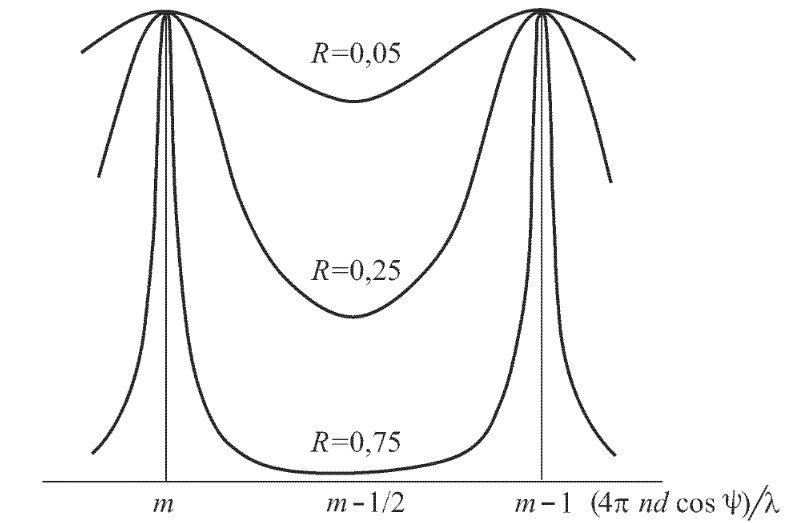
\includegraphics[width=0.3\textwidth]{figures/36_1.png}
    \caption{Пики для пластинки}
    \label{fig:piks}
\end{figure}
В окрестности максимума $m$-го порядка $\Phi = \pi m + \varphi$, тогда ввиду малости $\varphi$ можем написать
\begin{equation*}
    \sub{I}{d} = \frac{I_{\text{max}}}{1 + R \varphi^2/(1-R^2)},
    \hspace{0.5cm}
    \frac{R \varphi^2}{(1-R)^2} = 1 \text{ при } \sub{I}{d}= \frc{1}{2} \sub{I}{max},
    \hspace{0.5cm} \Rightarrow \hspace{0.5cm}
    \Delta \Phi = 2 \varphi = 2 \frac{1-R}{\sqrt{R}}.
\end{equation*}


\textbf{Разрешающая способность}. Имеем дело с интерференцией высоких порядков, поэтому требуется высокая \textit{монохроматичность света} ($\lambda/\delta \lambda \gg m$).

\begin{to_def}
    Разрешающая способность определяет наименьшее расстояние между близкими спектральными линиями, которые изображаются в виде раздельных спектральных линий. Если максимум одного пика находится не ближи полуширины другого, то их считают различимыми. 
\end{to_def}


Определим минимальную разность $\delta \lambda = \lambda'-\lambda$. Для интерферометра Фабри-Перо верно, что $n$ одинаков для двух длин волн. В точке $A'$ -- максимум $m$-го порядка для $\lambda'$, а потому $\Phi' = 2 \pi m$. В той же точке $\lambda$ имеет разность фаз $\Phi = 2 \pi m + (1-R)/\sqrt{R}$, т.е в рассматриваемой точке $\Phi'-\Phi = \delta \Phi = (1-R)/\sqrt{R}$. Но ввиду $n = n'$ верно, что $\delta \Phi / \Phi = |\delta \lambda / \lambda|$. Учтя, что в максимуме $\Phi = 2 \pi m$, находим
\begin{equation*}
    \frac{\lambda}{\delta \lambda} = \frac{2 \pi \sqrt{R}}{1-R} m, \text{ --- \textit{разрешающая способность спектрального прибора}.}
\end{equation*}



\textbf{Интерферометр Фабри-Перо}.
Он состоит из двух стеклянных 
или кварцевых пластинок $P_1$ и $P_2$, между которыми обычно находится воздух. Отражающая способность доводится до 95-98 \%, шероховатости допустимы в пределах $0.01 \lambda$. 
\begin{figure}[ht]
    \centering
    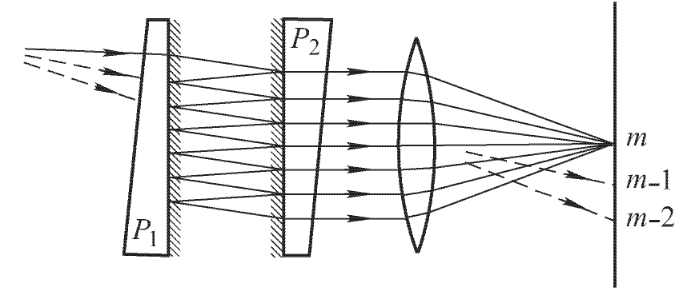
\includegraphics[width=0.5\textwidth]{figures/36_2.png}
    \caption{Интерферометр Фабри-Перо.}
    \label{fig:fp}
\end{figure}
Интерференционная картина состоит из концентрических колец равного наклона. Ввиду малости угла $\psi$ условие главного интерференционного максимума $2 h \cos \psi = m \lambda$ можно записать в виде $h(2-\psi^2) = m\lambda$ откуда \textit{угловая дисперсия} равна
\begin{equation*}
    \frac{d \psi}{d \lambda} = - \frac{m}{2 h \psi} = - \frac{1}{\lambda \psi},
\end{equation*}
которая значительно превышает дисперсию других спектральных приборов. 



\textbf{Интерферометр Фабри-Перо как резонатор}.
В этом разделе волны распространяются нормально к поверхности резонатора. Соответсвенно прибор прозрачен для длин вол излучения, удовлетворяющих условию $m \lambda = 2 L$. Также $L$ -- расстояние между зеркалами $\gg \lambda$, а также $1-R \ll 1$. Добротность запишем, как
\begin{equation*}
    Q = 2 \pi \frac{E_0}{\Delta E}, 
\end{equation*}
где $E_0$ -- накопленная энергия, а $\Delta E$ -- энергия, теряемая за период колебаний. 
В указанных предположениях верно, что есть стоячая волна, эквивалентная суперпозиции двух бегущих. 



\begin{to_def}
    \textit{Резонатор} -- колебательная система, устройство, способное накапливать энергию колебаний, поставляемую из внешнего источника. 
\end{to_def}


Если поток энергии в каждой их волн равен $P$, то энергия равна 
\begin{equation*}
    E_0 = 2 P \tau_L = 2 P L/c,
\end{equation*}
где $\tau_L = L/c$ -- время, за которое волна проходит расстояние $L$ между пластинами. Поскольку можность потерь составляет $(1-R) 2 P$, то за период колебаний $T$ теряется энергия 
\begin{equation*}
    \Delta E = 2 P (1-R) T.
\end{equation*}
Так как $\lambda = c T$, то по определению находим
\begin{equation*}
    Q = 2 \pi \frac{E_0}{\Delta E_0} = 2 \pi \frac{L}{\lambda} \frac{1}{1-R}.
\end{equation*}
Зная добротность, мы можем найти эффективную ширину линии излучения, выходящего из резонатора:
$\Delta \sub{\lambda}{eff} = \lambda/Q$, по определению добротности $Q = \omega / \Delta \omega$, преобразованного с помощью равенства $\Delta/\omega = \Delta \lambda/\lambda$ вытекающего из $\omega = 2 \pi c / \lambda$. В таком случае приходим к формуле вида
\begin{equation*}
    \Delta \lambda = \lambda \frac{\Delta \nu}{\nu} = \frac{\lambda^2}{2L}.
\end{equation*}
Таким образом выделяемые резонатором линии являются в высокой степени монохроматическими. 

Теперь читателю предоставляется прочитать текст идущий далее, а потом вернуться к этим строчкам, где я опишу интерферометр Фабри-Перо как спектральный прибор.
Если он у нас заполнен однородной однородной средой с показателем преломления $n$. То разрешающая способность даётся как
\begin{equation*}
    R = \frac{\lambda}{\delta\lambda} = \frac{2 \pi \sqrt{R} m}{1 - R}\left(1 - \frac{1}{\cos^2 \psi} \frac{\lambda}{n} \frac{d n}{d \lambda}\right).
\end{equation*}